\documentclass[12pt]{article}
\usepackage{fullpage,graphicx,psfrag,amsmath,amsfonts,verbatim}
\usepackage[small,bf]{caption}
\usepackage{float}

\input defs.tex

\bibliographystyle{alpha}

\title{Assignment 4 CME 241}
\author{Taylor Howell}

\begin{document}
\maketitle

\newpage
\section*{1. Manual Value Iteration}
\begin{figure}[!htb]
	\centering
	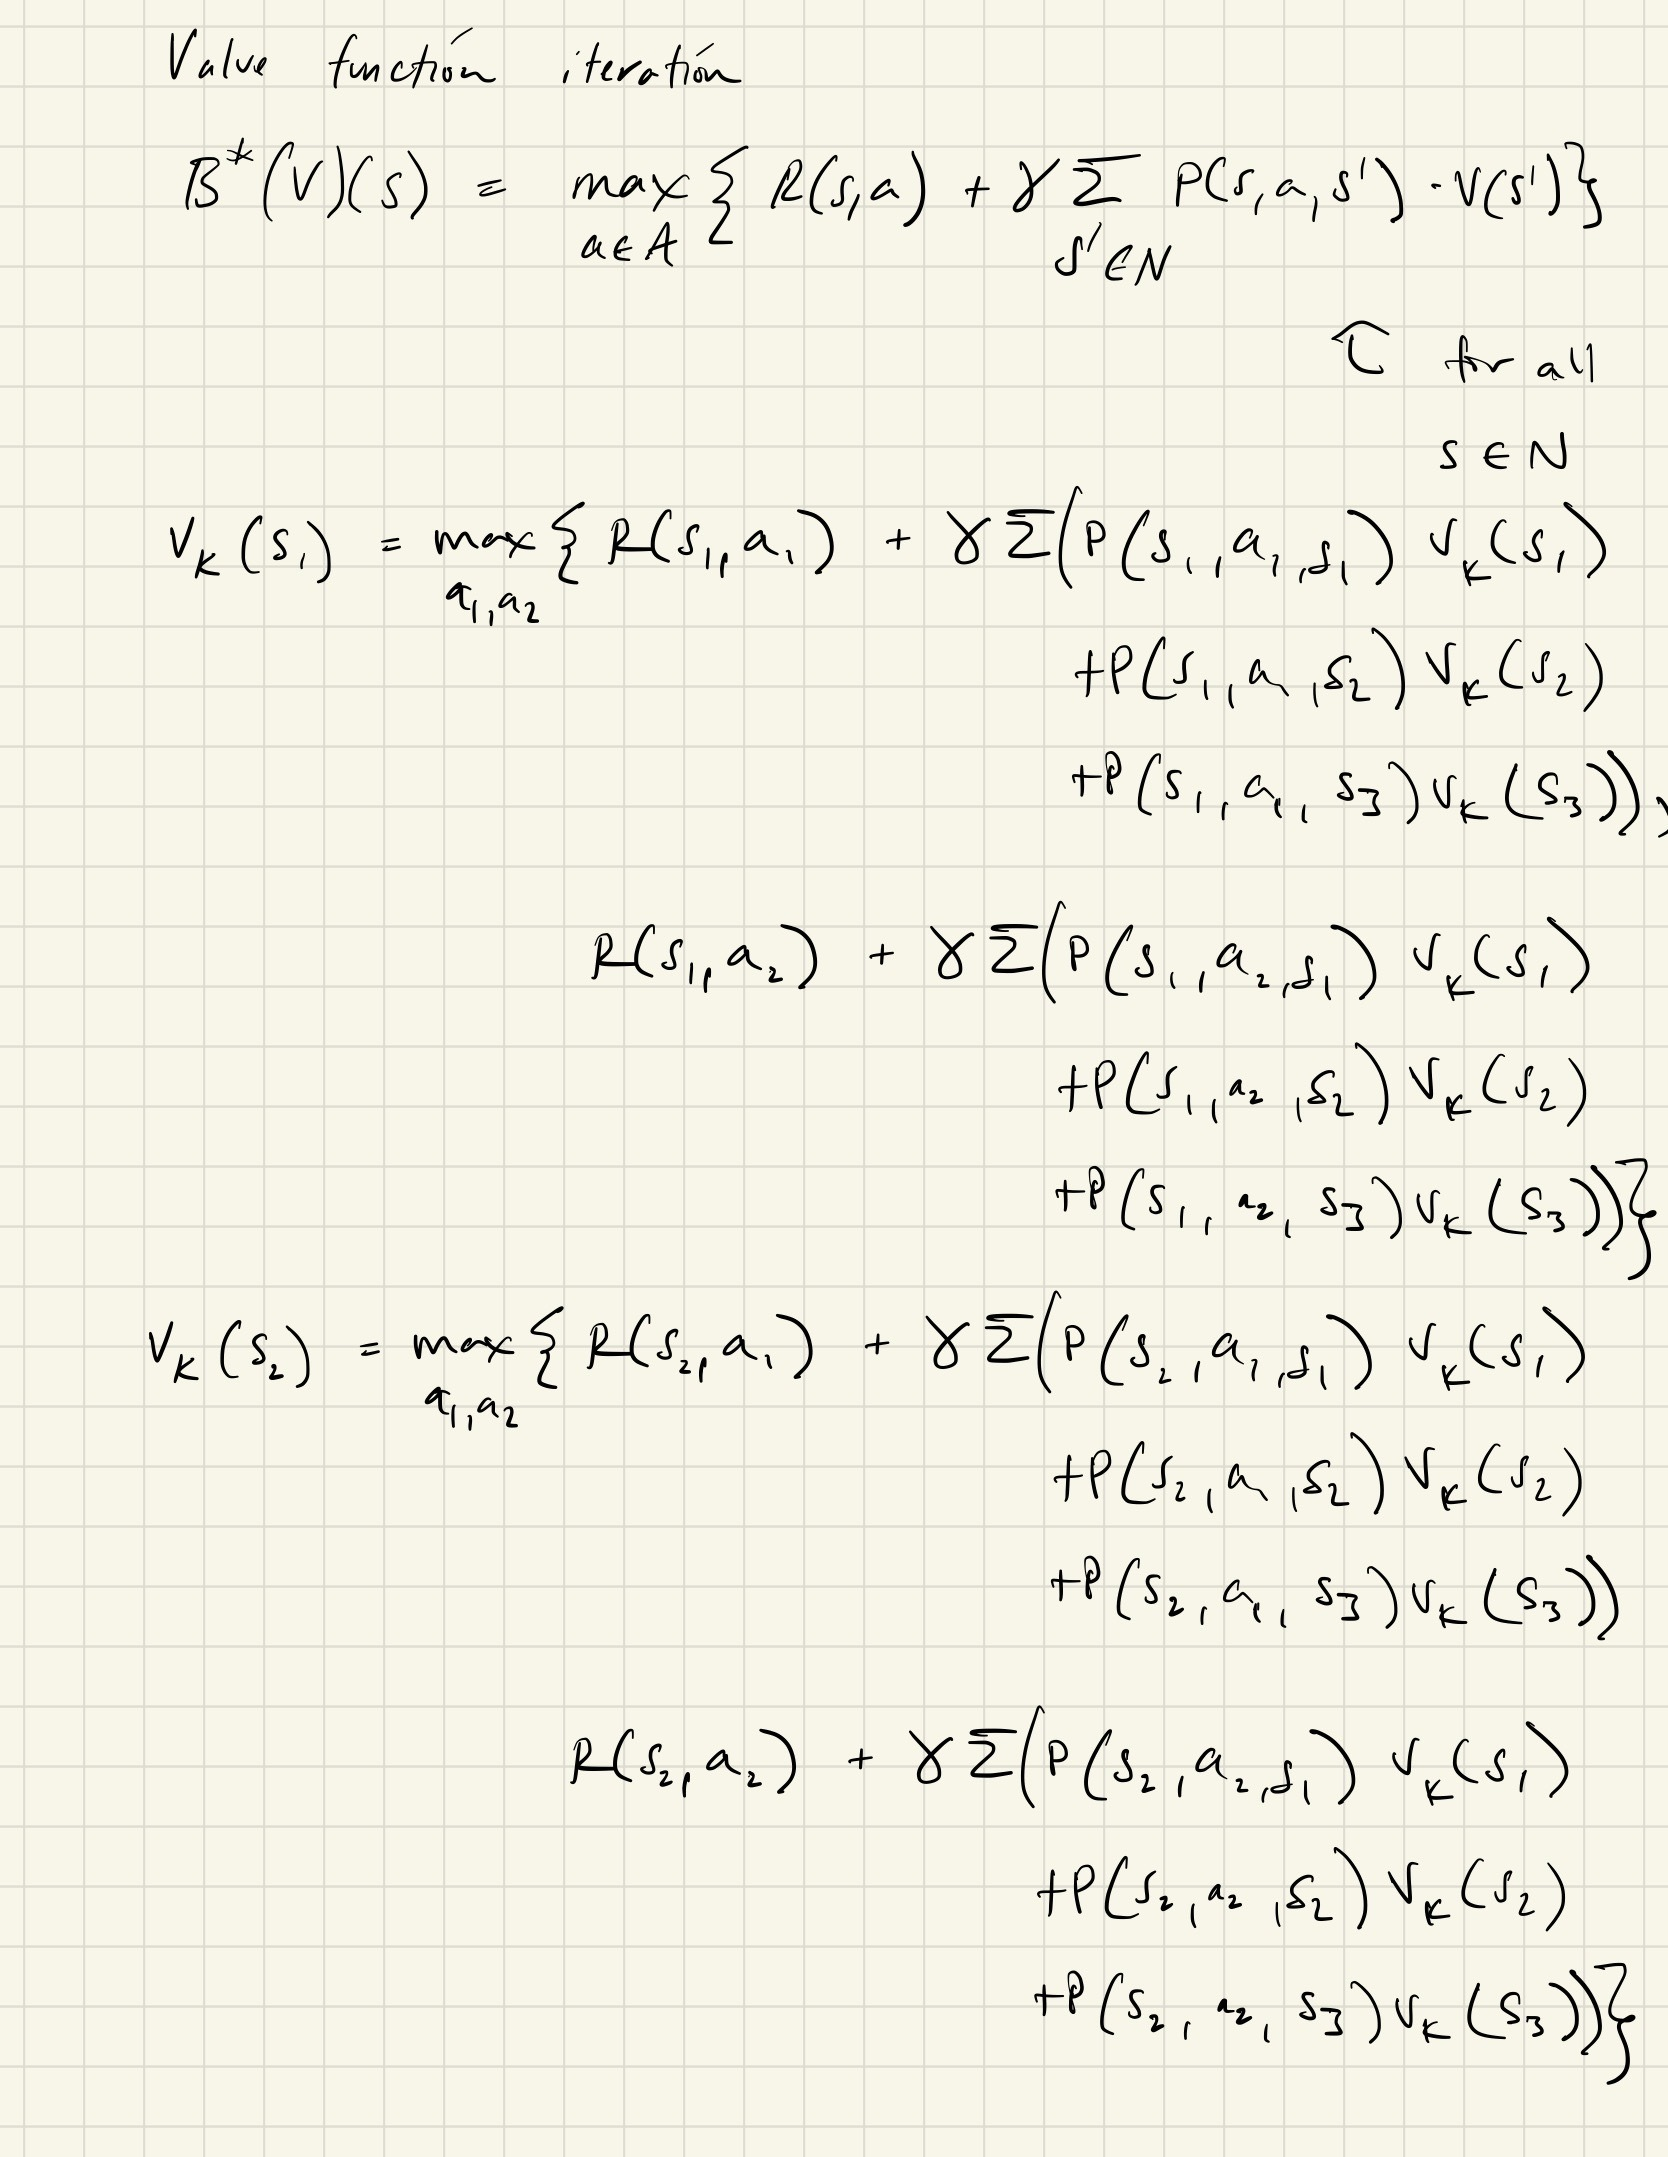
\includegraphics[width=.75\textwidth]{ipad/q1_1.jpg}
\end{figure}

\begin{figure}[!htb]
	\centering
	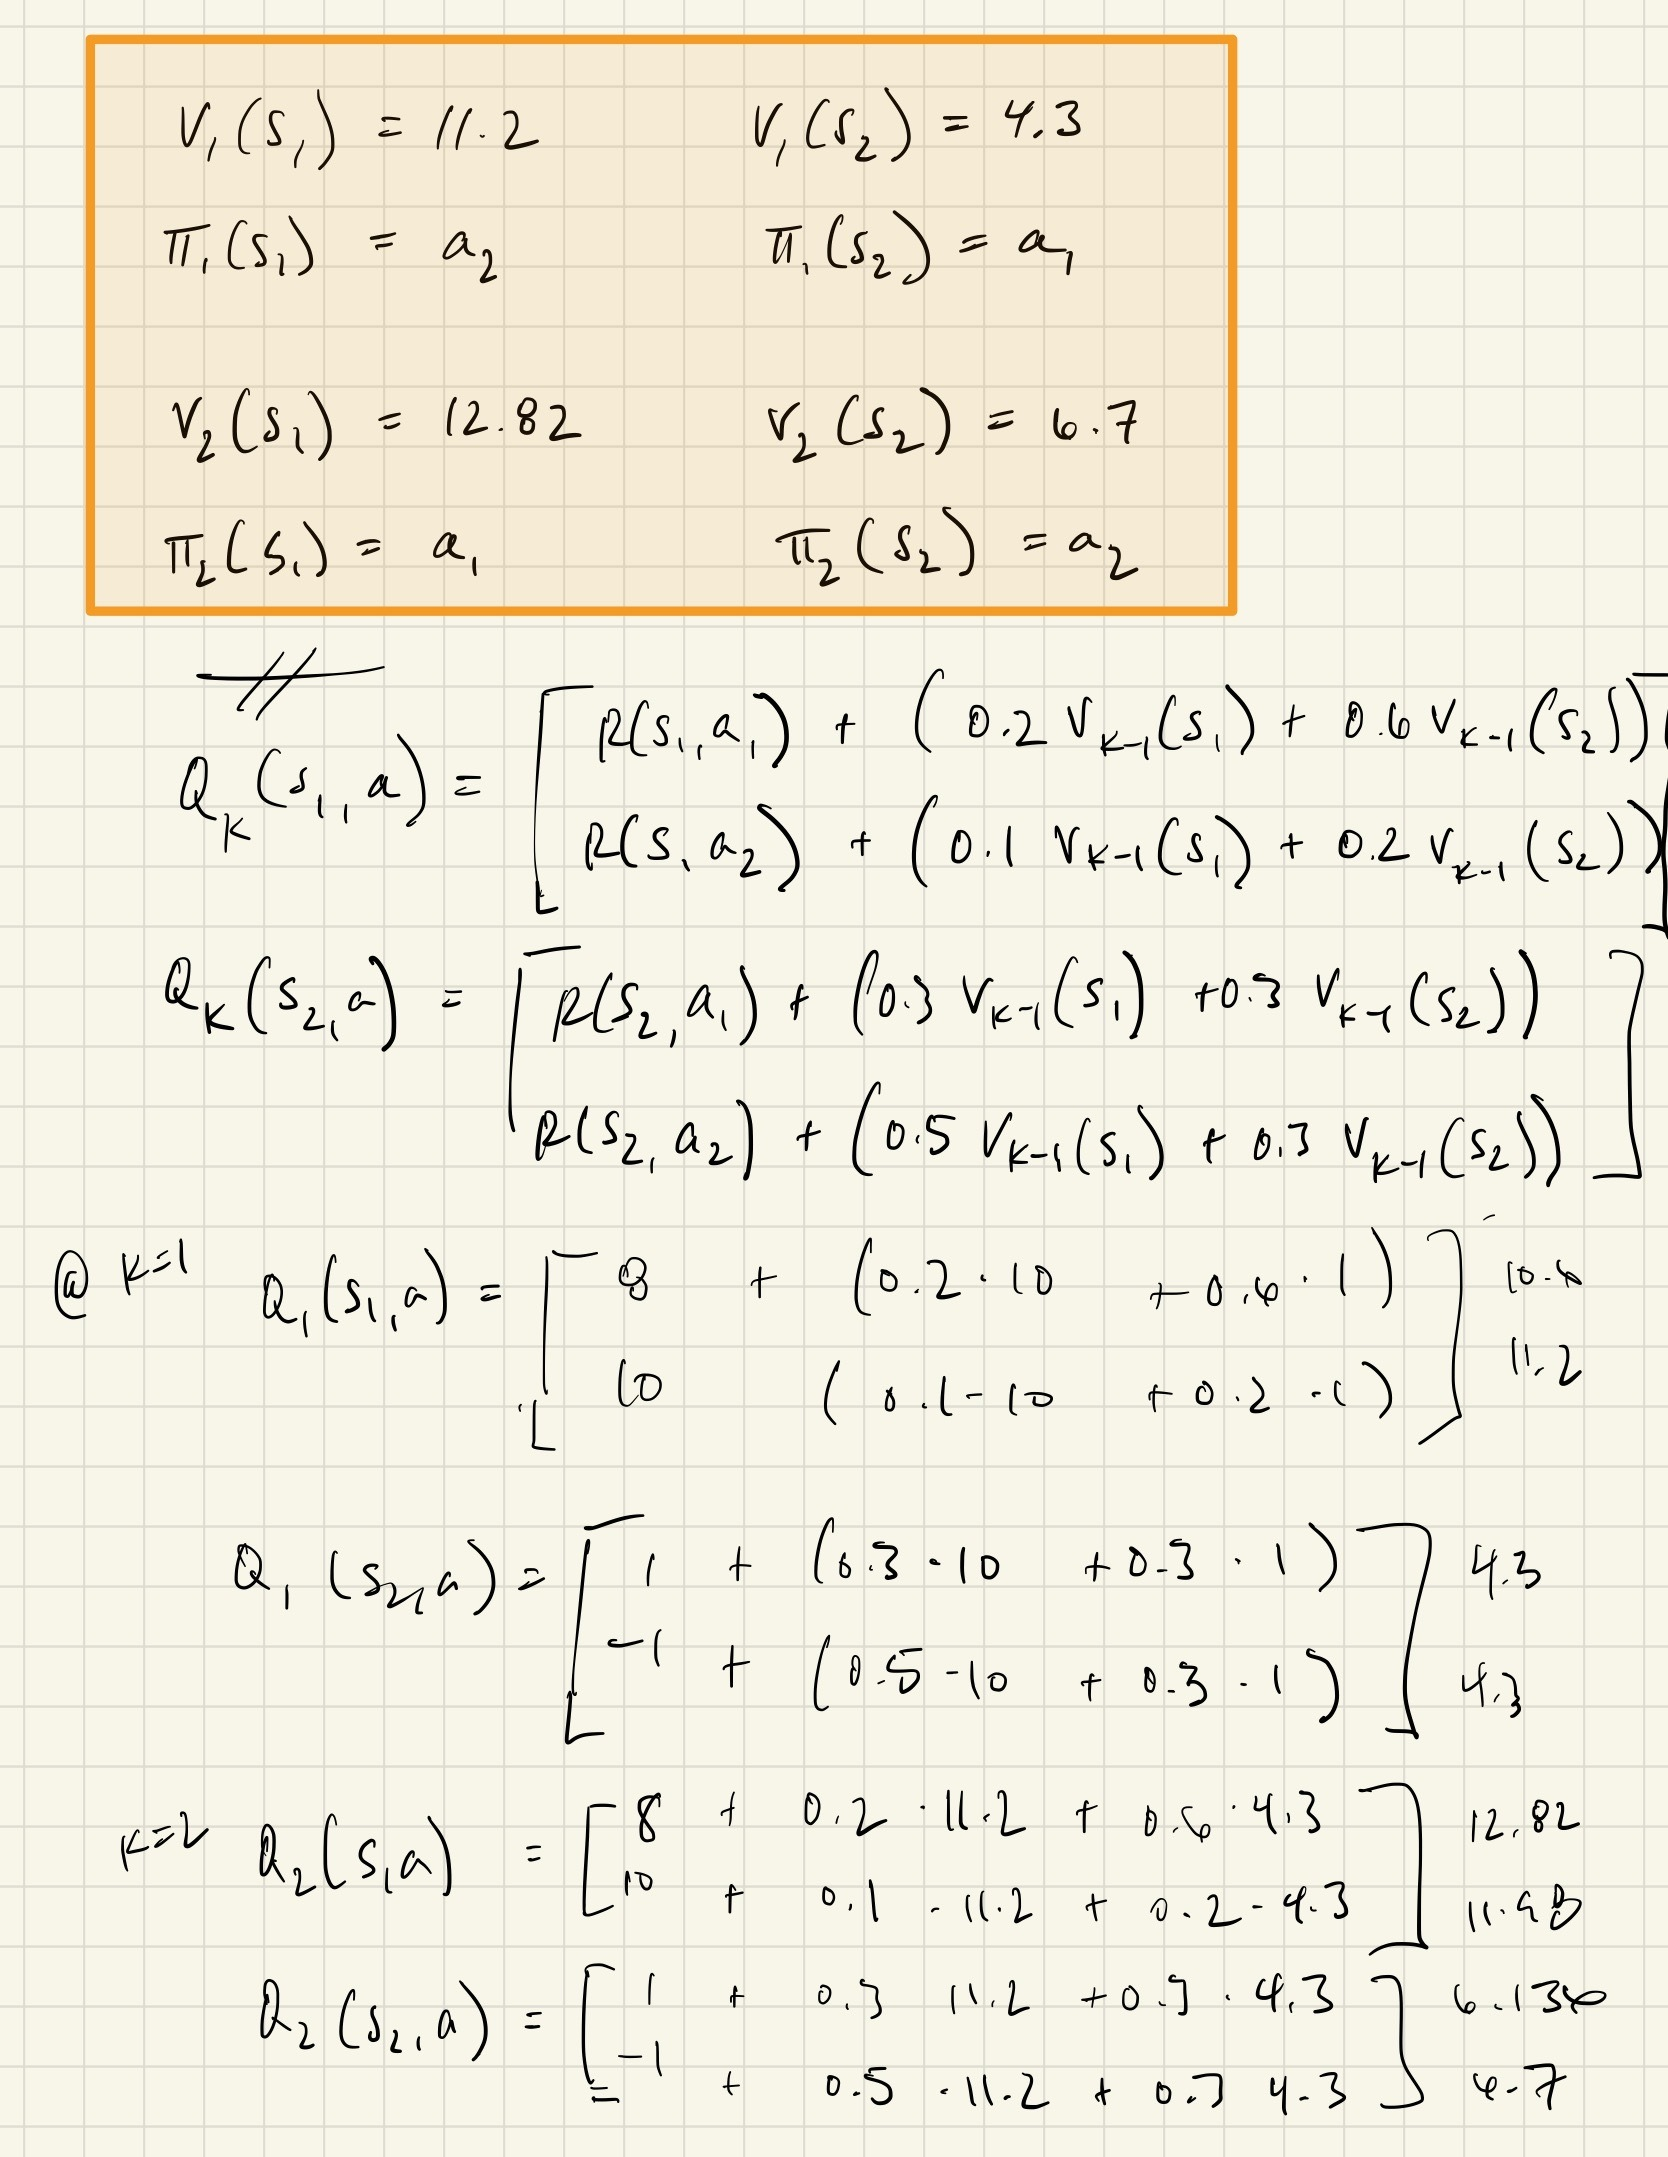
\includegraphics[width=.75\textwidth]{ipad/q1_2.jpg}
\end{figure}

\begin{figure}[!htb]
	\centering
	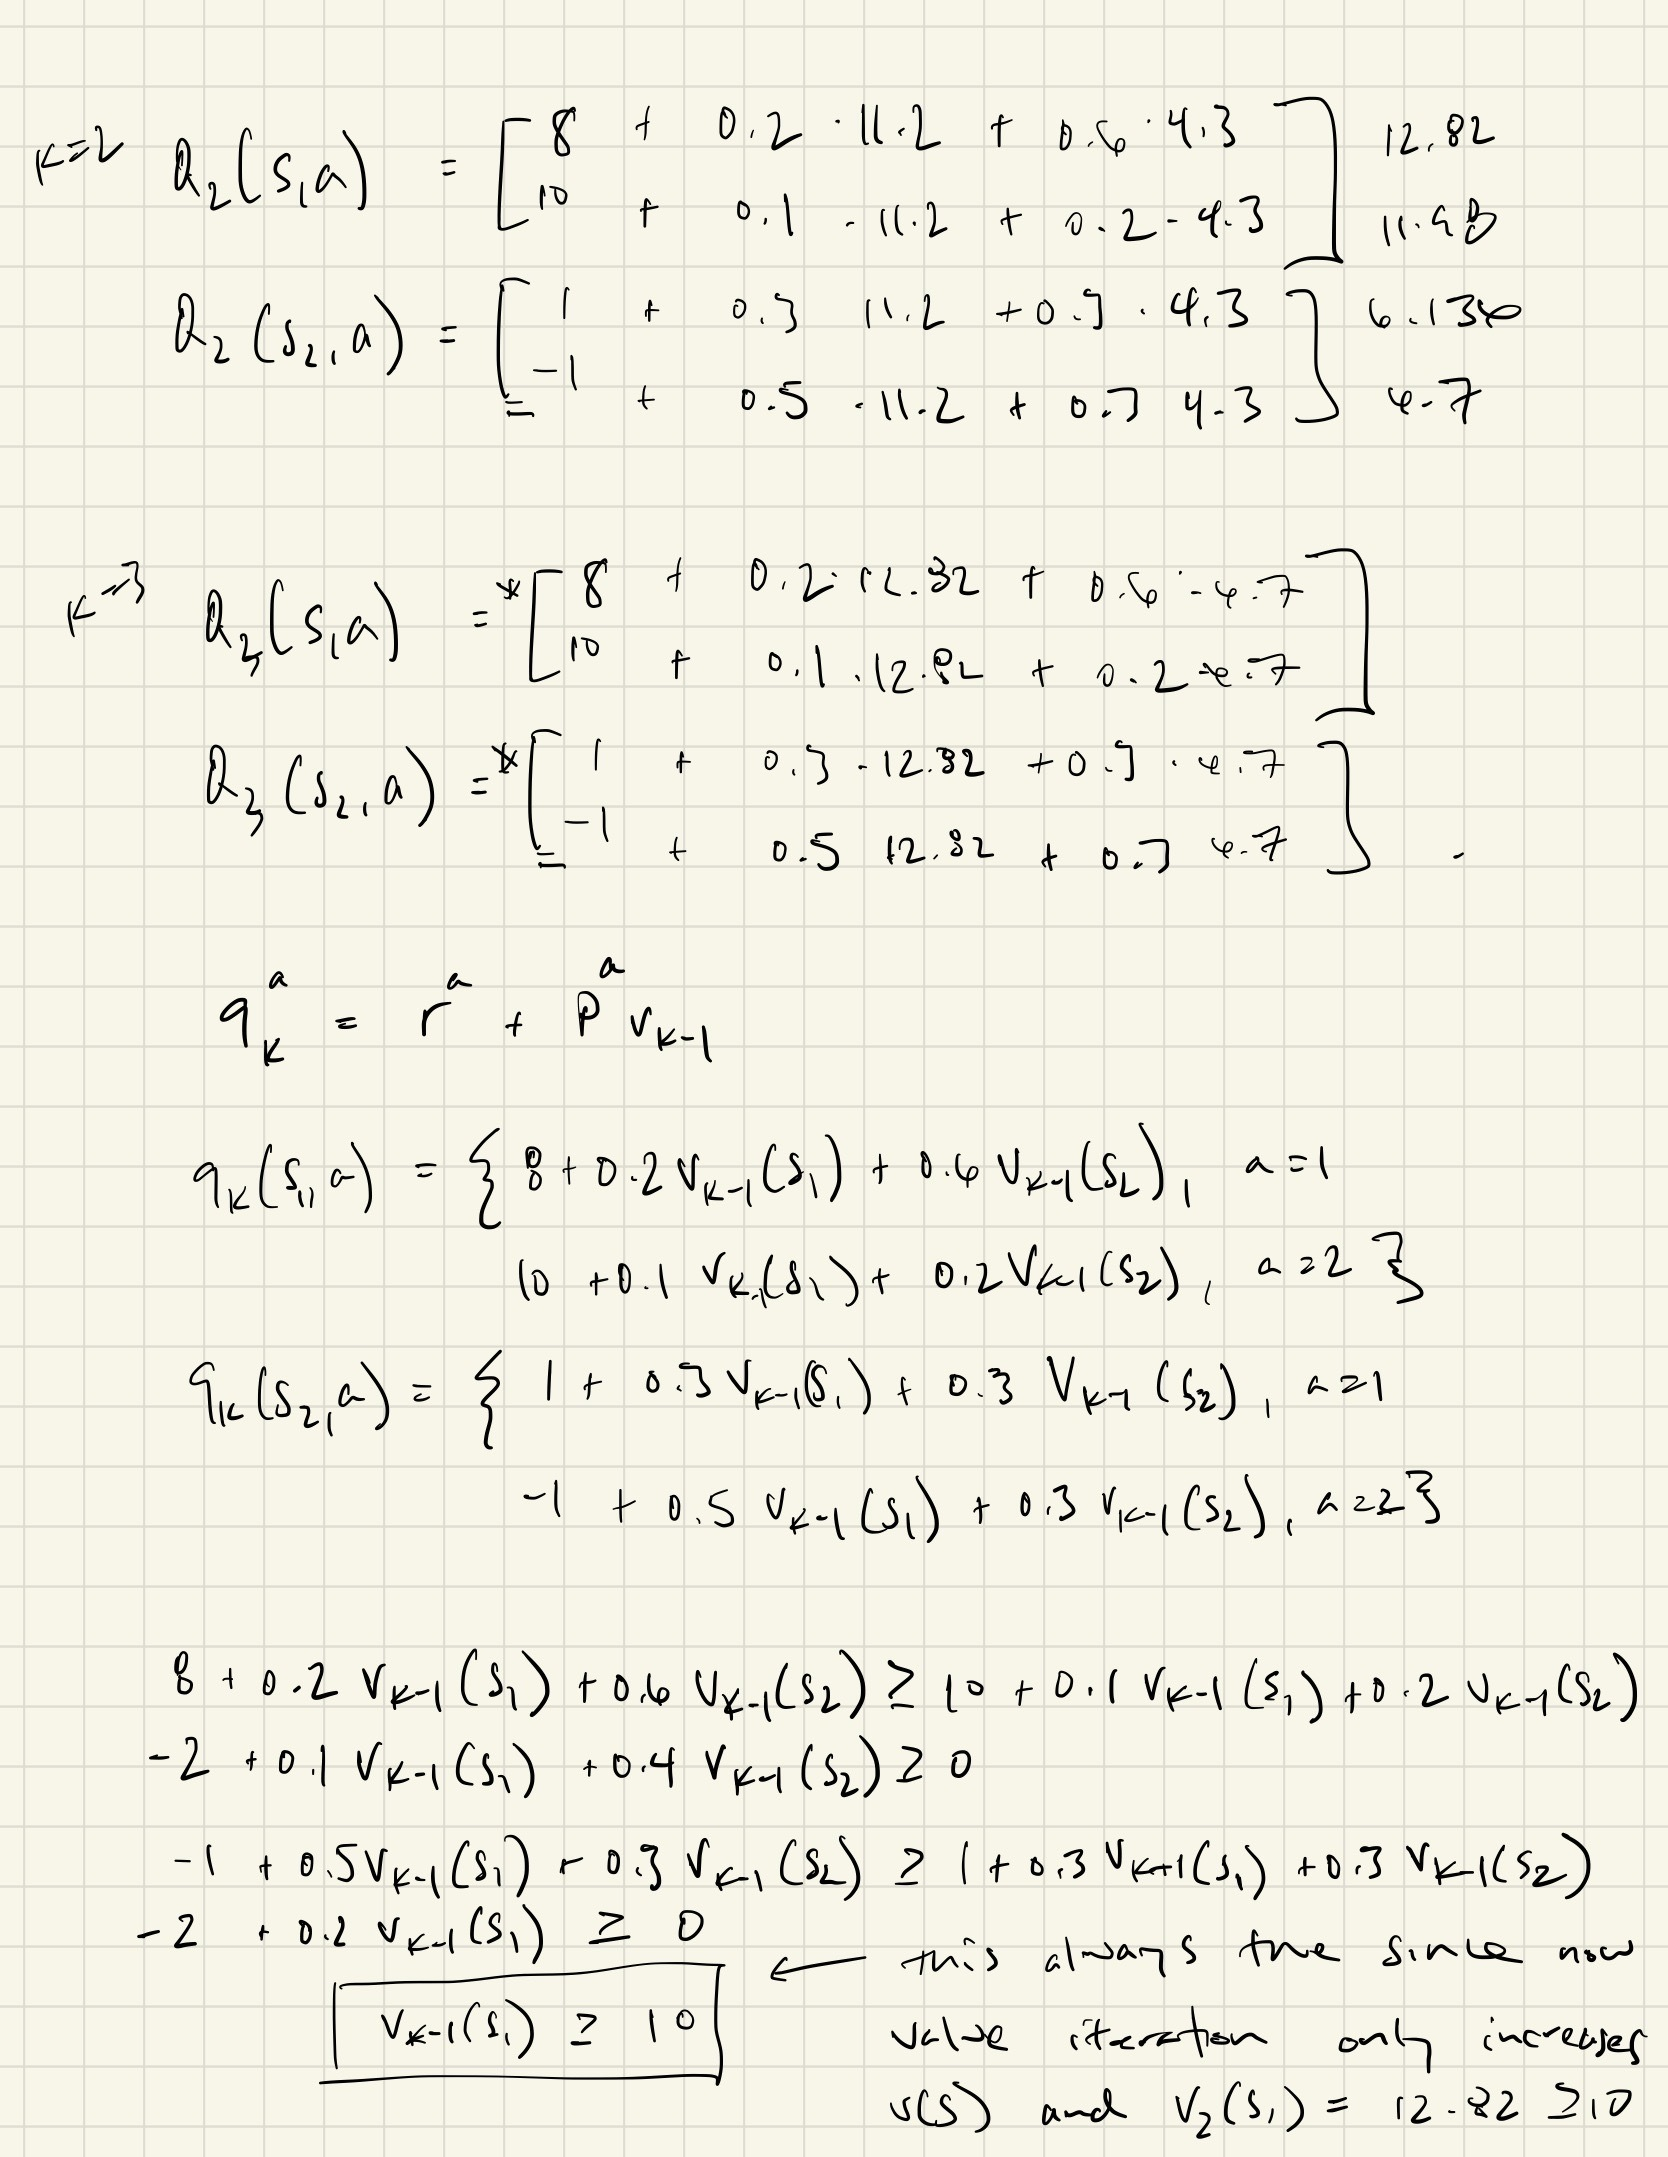
\includegraphics[width=.75\textwidth]{ipad/q1_3.jpg}
\end{figure}

\begin{figure}[!htb]
	\centering
	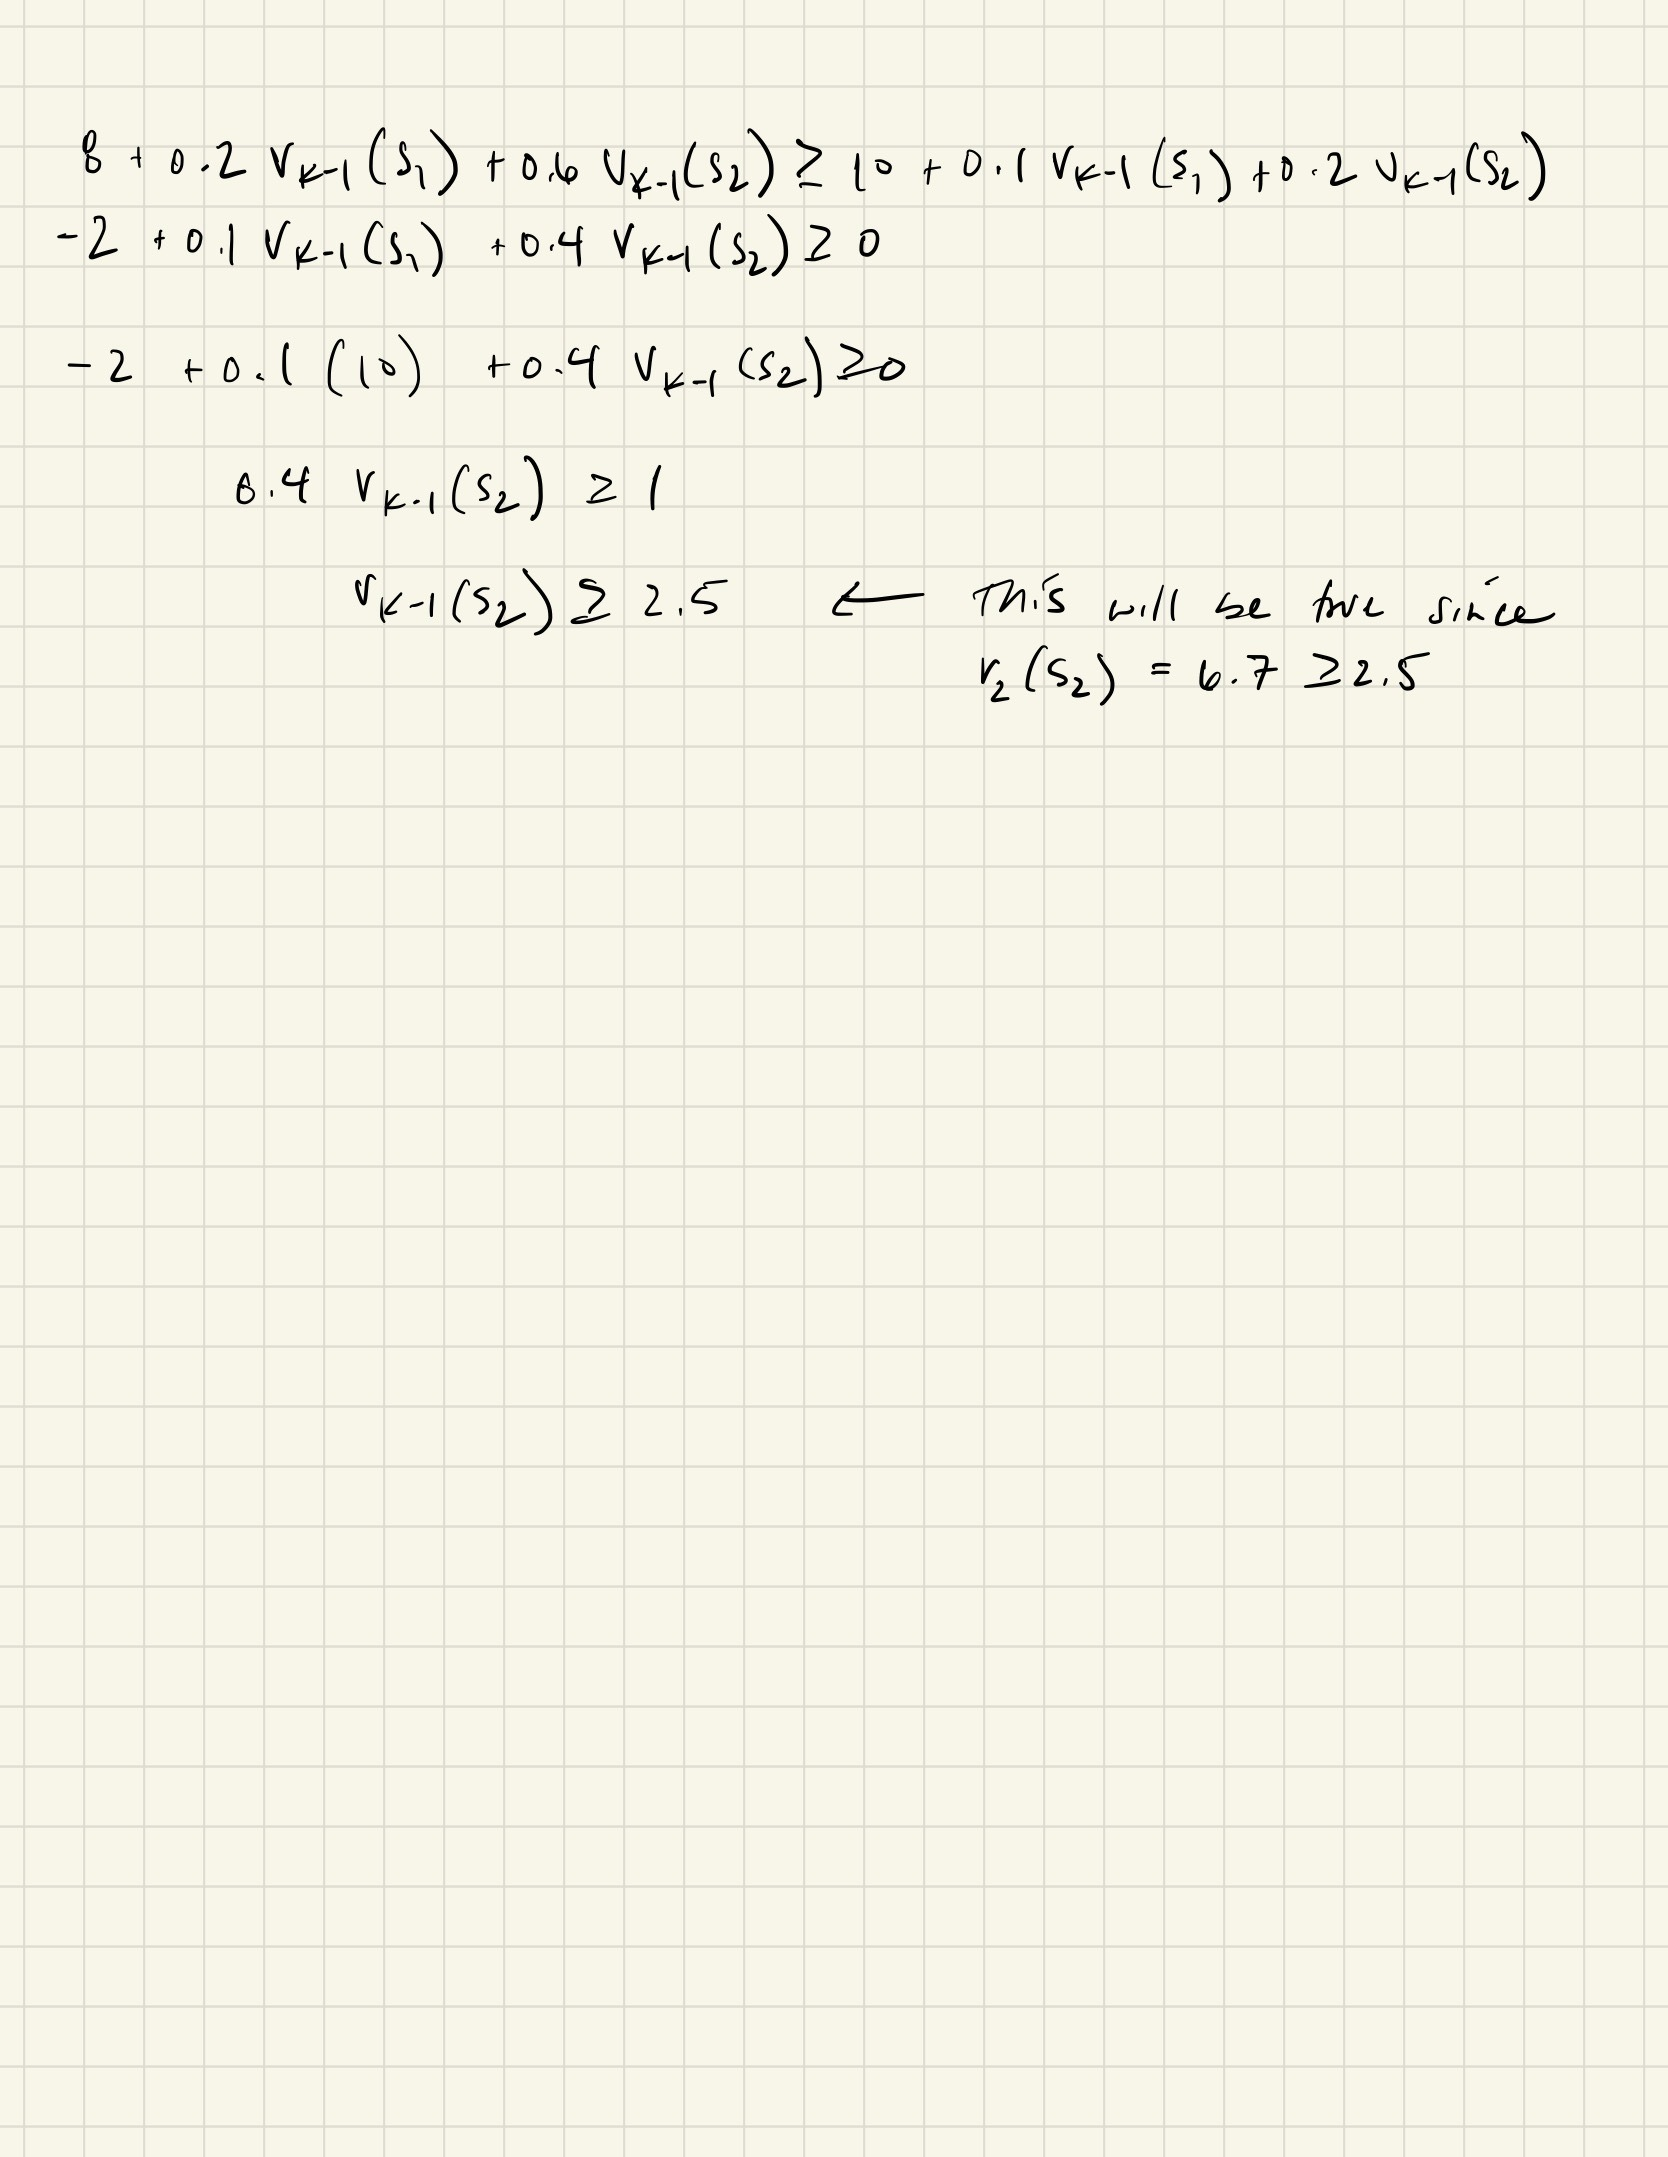
\includegraphics[width=.75\textwidth]{ipad/q1_4.jpg}
\end{figure}

\clearpage
\section*{2. Frog Croaking revisited}
For this problem, I have reimplemented my MDP in Julia (see \texttt{frog\_escape.jl}). Additionally, I have implemented value iteration (\texttt{value\_iteration.jl}) and policy iteration (\texttt{policy\_iteration.jl}) from scratch.

I also remodeled the reward function since the last assignment:
$$\mathcal{R}(s, a) = 1 \cdot \mathcal{P}(S_t = s, A_t = a, S_{t+1} = n)$$

%\begin{figure}
%	\centering
%	\includegraphics[width=.5\textwidth]{}
%\end{figure}

\end{document}
